\subsection{Instancias de pruebas}



En el  \cite{Yuan20091081} se presenta un red de 20 nodos divididos en 3 áreas que se muestra en la figura \ref{area3}. En cada área los parámetros son generados de forma aleatoria, los cuales se observan en el cuadro \ref{table:intervalo}. Para el desastre 0 es una situación sin ningún desastre y el desastre 4 es situación más compleja. Para las instancias propuesta por \cite{Yuan20091081} se considera que el nodo 20 es un nodo seguro.

\begin{figure}[H]
\centering
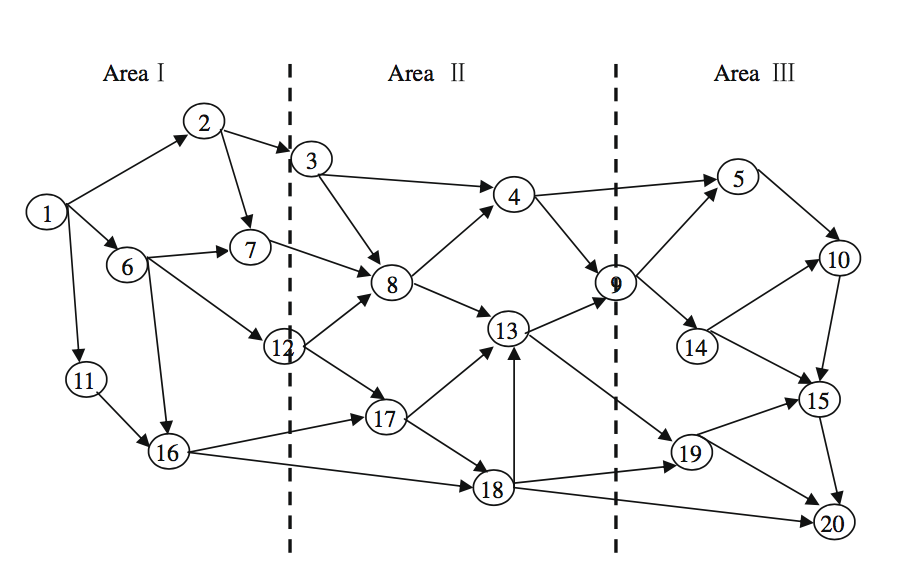
\includegraphics[scale=0.5]{images/areas.jpg}
\caption{División de una red de emergencia}\label{area3}

\end{figure}

En los cuadros \ref{grade1}, \ref{grade2}, \ref{grade3} y \ref{grade4} se muestran los valores correspondientes al nodo $i$ y nodo $j$. $l_{i,j}$ $s_{i,j}^0$, $\alpha_{ij}$ y $\beta_{ij}$ según los distintos grados de desastre.



\begin{table}[H]
\centering
\begin{tabular}{|l|l|l|l|}
\hline
Tipo & Área I & Área II & Área III \\ \hline
Desastre 0 & $\alpha=1$,$\beta=0$ & $\alpha=1$,$\beta=0$ & $\alpha=1$,$\beta=0$ \\ \hline
Desastre 1 & $\alpha \in (0.9,1.0)$ $\beta \in (0.00,0.05)$ & $\alpha=1$,$\beta=0$ & $\alpha=1$,$\beta=0$ \\ \hline
Desastre 2 & $\alpha \in (0.8,0.9)$ $\beta \in (0.05,0.10)$ & $\alpha \in (0.9,1.0)$ $\beta \in (0.00,0.05)$ & $\alpha=1$,$\beta=0$ \\ \hline
Desastre 3 & $\alpha \in (0.7,0.8)$ $\beta \in (0.10,0.15)$ & $\alpha \in (0.8,0.9)$ $\beta \in (0.05,0.10)$ & $\alpha \in (0.9,1.0)$ $\beta \in (0.00,0.05)$ \\ \hline
Desastre 4 & $\alpha \in (0.6,0.7)$ $\beta \in (0.15,0.20)$ & $\alpha \in (0.7,0.8)$ $\beta \in (0.10,0.15)$ & $\alpha \in (0.8,0.9)$ $\beta \in (0.05,0.10)$ \\ \hline
\end{tabular}
\caption{Intervalos de los parametros por área}\label{table:intervalo}
\end{table}




\begin{table}[H]
\centering
\begin{tabular}{|l|l|l|l|l|l|}
\hline
inicio & fin & $l_{i,j}$ & $s_{i,j}^0$ & $\alpha_{i,j}$ & $\beta_{i,j}$ \\ \hline
1 & 2 & 50 & 100 & 0.9222 & 0.0381 \\ \hline
1 & 6 & 30 & 60 & 0.9193 & 0.0143 \\ \hline
1 & 11 & 70 & 110 & 0.9022 & 0.0499 \\ \hline
2 & 3 & 30 & 60 & 0.9904 & 0.0277 \\ \hline
2 & 7 & 40 & 70 & 0.9857 & 0.0305 \\ \hline
6 & 7 & 30 & 65 & 0.9577 & 0.0123 \\ \hline
6 & 12 & 60 & 105 & 0.906 & 0.0399 \\ \hline
6 & 16 & 100 & 115 & 0.9049 & 0.0353 \\ \hline
7 & 8 & 40 & 90 & 0.9153 & 0.0436 \\ \hline
11 & 16 & 30 & 70 & 0.9967 & 0.0089 \\ \hline
16 & 17 & 80 & 115 & 0.964 & 0.0491 \\ \hline
16 & 18 & 110 & 120 & 0.9294 & 0.0327 \\ \hline
3 & 4 & 80 & 100 & 1 & 0 \\ \hline
3 & 8 & 60 & 95 & 1 & 0 \\ \hline
4 & 5 & 110 & 120 & 1 & 0 \\ \hline
4 & 9 & 40 & 75 & 1 & 0 \\ \hline
5 & 10 & 60 & 110 & 1 & 0 \\ \hline
8 & 4 & 40 & 85 & 1 & 0 \\ \hline
8 & 13 & 30 & 75 & 1 & 0 \\ \hline
9 & 5 & 70 & 110 & 1 & 0 \\ \hline
9 & 14 & 40 & 90 & 1 & 0 \\ \hline
10 & 15 & 50 & 105 & 1 & 0 \\ \hline
12 & 8 & 30 & 65 & 1 & 0 \\ \hline
12 & 17 & 40 & 100 & 1 & 0 \\ \hline
13 & 9 & 30 & 80 & 1 & 0 \\ \hline
13 & 19 & 110 & 120 & 1 & 0 \\ \hline
14 & 10 & 80 & 115 & 1 & 0 \\ \hline
14 & 15 & 60 & 105 & 1 & 0 \\ \hline
15 & 20 & 30 & 90 & 1 & 0 \\ \hline
17 & 13 & 40 & 80 & 1 & 0 \\ \hline
17 & 18 & 40 & 75 & 1 & 0 \\ \hline
18 & 13 & 60 & 115 & 1 & 0 \\ \hline
18 & 19 & 70 & 110 & 1 & 0 \\ \hline
18 & 20 & 120 & 120 & 1 & 0 \\ \hline
19 & 15 & 40 & 75 & 1 & 0 \\ \hline
19 & 20 & 70 & 105 & 1 & 0 \\ \hline

\end{tabular}
\caption{Parámetros para un desastre grado 1}
\label{grade1}
\end{table}


\begin{table}[H]
\centering
\begin{tabular}{|l|l|l|l|l|l|}
\hline
inicio & fin & $l_{i,j}$ & $s_{i,j}^0$ & $\alpha_{i,j}$ & $\beta_{i,j}$ \\ \hline
1 & 2 & 50 & 100 & 0.9222 & 0.0381 \\ \hline
1 & 6 & 30 & 60 & 0.9193 & 0.0143 \\ \hline
1 & 11 & 70 & 110 & 0.9022 & 0.0499 \\ \hline
2 & 3 & 30 & 60 & 0.9904 & 0.0277 \\ \hline
2 & 7 & 40 & 70 & 0.9857 & 0.0305 \\ \hline
6 & 7 & 30 & 65 & 0.9577 & 0.0123 \\ \hline
6 & 12 & 60 & 105 & 0.906 & 0.0399 \\ \hline
6 & 16 & 100 & 115 & 0.9049 & 0.0353 \\ \hline
7 & 8 & 40 & 90 & 0.9153 & 0.0436 \\ \hline
11 & 16 & 30 & 70 & 0.9967 & 0.0089 \\ \hline
16 & 17 & 80 & 115 & 0.964 & 0.0491 \\ \hline
16 & 18 & 110 & 120 & 0.9294 & 0.0327 \\ \hline
3 & 4 & 80 & 100 & 0.9153 & 0.0216 \\ \hline
3 & 8 & 60 & 95 & 0.9562 & 0.0114 \\ \hline
4 & 5 & 110 & 120 & 0.989 & 0.0281 \\ \hline
4 & 9 & 40 & 75 & 0.9984 & 0.0386 \\ \hline
8 & 4 & 40 & 85 & 0.9746 & 0.0376 \\ \hline
8 & 13 & 30 & 75 & 0.9999 & 0.0222 \\ \hline
12 & 8 & 30 & 65 & 0.9345 & 0.0044 \\ \hline
12 & 17 & 40 & 100 & 0.9846 & 0.0228 \\ \hline
13 & 9 & 30 & 80 & 0.9094 & 0.0264 \\ \hline
13 & 19 & 110 & 120 & 0.9326 & 0.0151 \\ \hline
17 & 13 & 40 & 80 & 0.9077 & 0.035 \\ \hline
17 & 18 & 40 & 75 & 0.947 & 0.0344 \\ \hline
18 & 13 & 60 & 115 & 0.9669 & 0.0202 \\ \hline
18 & 19 & 70 & 110 & 0.953 & 0.0059 \\ \hline
18 & 20 & 120 & 120 & 0.9278 & 0.0021 \\ \hline
5 & 10 & 60 & 110 & 1 & 0 \\ \hline
9 & 5 & 70 & 110 & 1 & 0 \\ \hline
9 & 14 & 40 & 90 & 1 & 0 \\ \hline
10 & 15 & 50 & 105 & 1 & 0 \\ \hline
14 & 10 & 80 & 115 & 1 & 0 \\ \hline
14 & 15 & 60 & 105 & 1 & 0 \\ \hline
15 & 20 & 30 & 90 & 1 & 0 \\ \hline
19 & 15 & 40 & 75 & 1 & 0 \\ \hline
19 & 20 & 70 & 105 & 1 & 0 \\ \hline
\end{tabular}
\caption{Parámetros para un desastre grado 2}
\label{grade2}
\end{table}

\begin{table}[H]
\centering
\begin{tabular}{|l|l|l|l|l|l|}
\hline
inicio & fin & $l_{i,j}$ & $s_{i,j}^0$ & $\alpha_{i,j}$ & $\beta_{i,j}$ \\ \hline
1 & 2 & 50 & 100 & 0.7544 & 0.1026 \\ \hline
1 & 6 & 30 & 60 & 0.7666 & 0.1394 \\ \hline
1 & 11 & 70 & 110 & 0.7561 & 0.1276 \\ \hline
2 & 3 & 30 & 60 & 0.7071 & 0.1089 \\ \hline
2 & 7 & 40 & 70 & 0.7527 & 0.1277 \\ \hline
6 & 7 & 30 & 65 & 0.7001 & 0.1062 \\ \hline
6 & 12 & 60 & 105 & 0.7145 & 0.1209 \\ \hline
6 & 16 & 100 & 115 & 0.7234 & 0.1361 \\ \hline
7 & 8 & 40 & 90 & 0.7242 & 0.108 \\ \hline
11 & 16 & 30 & 70 & 0.7378 & 0.1281 \\ \hline
16 & 17 & 80 & 115 & 0.7048 & 0.1197 \\ \hline
16 & 18 & 110 & 120 & 0.7639 & 0.1365 \\ \hline
3 & 4 & 80 & 100 & 0.8912 & 0.0844 \\ \hline
3 & 8 & 60 & 95 & 0.8242 & 0.0571 \\ \hline
4 & 5 & 110 & 120 & 0.8773 & 0.0552 \\ \hline
4 & 9 & 40 & 75 & 0.8678 & 0.099 \\ \hline
8 & 4 & 40 & 85 & 0.8801 & 0.067 \\ \hline
8 & 13 & 30 & 75 & 0.8425 & 0.0987 \\ \hline
12 & 8 & 30 & 65 & 0.8383 & 0.0543 \\ \hline
12 & 17 & 40 & 100 & 0.8785 & 0.0786 \\ \hline
13 & 9 & 30 & 80 & 0.8551 & 0.0707 \\ \hline
13 & 19 & 110 & 120 & 0.873 & 0.057 \\ \hline
17 & 13 & 40 & 80 & 0.8191 & 0.0778 \\ \hline
17 & 18 & 40 & 75 & 0.8555 & 0.0781 \\ \hline
18 & 13 & 60 & 115 & 0.8965 & 0.0653 \\ \hline
18 & 19 & 70 & 110 & 0.8967 & 0.0694 \\ \hline
18 & 20 & 120 & 120 & 0.8551 & 0.0948 \\ \hline
5 & 10 & 60 & 110 & 0.9476 & 0.0343 \\ \hline
9 & 5 & 70 & 110 & 0.9806 & 0.0484 \\ \hline
9 & 14 & 40 & 90 & 0.9984 & 0.0219 \\ \hline
10 & 15 & 50 & 105 & 0.9937 & 0.0091 \\ \hline
14 & 10 & 80 & 115 & 0.9334 & 0.0486 \\ \hline
14 & 15 & 60 & 105 & 0.9966 & 0.022 \\ \hline
15 & 20 & 30 & 90 & 0.9517 & 0.0363 \\ \hline
19 & 15 & 40 & 75 & 0.9547 & 0.0265 \\ \hline
19 & 20 & 70 & 105 & 0.9849 & 0.029 \\ \hline
\end{tabular}
\caption{Parámetros para un desastre grado 3}\label{grade3}
\end{table}


\begin{table}[H]
\centering
\begin{tabular}{|l|l|l|l|l|l|}
\hline
inicio & fin & $l_{i,j}$ & $s_{i,j}^0$ & $\alpha_{i,j}$ & $\beta_{i,j}$ \\ \hline
1 & 2 & 50 & 100 & 0.6396 & 0.1783 \\ \hline
1 & 6 & 30 & 60 & 0.6815 & 0.1934 \\ \hline
1 & 11 & 70 & 110 & 0.6204 & 0.1647 \\ \hline
2 & 3 & 30 & 60 & 0.6244 & 0.1698 \\ \hline
2 & 7 & 40 & 70 & 0.658 & 0.1674 \\ \hline
6 & 7 & 30 & 65 & 0.6481 & 0.1515 \\ \hline
6 & 12 & 60 & 105 & 0.6717 & 0.1957 \\ \hline
6 & 16 & 100 & 115 & 0.6706 & 0.1672 \\ \hline
7 & 8 & 40 & 90 & 0.6619 & 0.1864 \\ \hline
11 & 16 & 30 & 70 & 0.6821 & 0.1645 \\ \hline
16 & 17 & 80 & 115 & 0.6146 & 0.1858 \\ \hline
16 & 18 & 110 & 120 & 0.6625 & 0.1918 \\ \hline
3 & 4 & 80 & 100 & 0.7606 & 0.1184 \\ \hline
3 & 8 & 60 & 95 & 0.7454 & 0.1348 \\ \hline
4 & 5 & 110 & 120 & 0.7276 & 0.1178 \\ \hline
4 & 9 & 40 & 75 & 0.7686 & 0.1192 \\ \hline
8 & 4 & 40 & 85 & 0.7416 & 0.1484 \\ \hline
8 & 13 & 30 & 75 & 0.7073 & 0.132 \\ \hline
12 & 8 & 30 & 65 & 0.7911 & 0.1081 \\ \hline
12 & 17 & 40 & 100 & 0.7222 & 0.117 \\ \hline
13 & 9 & 30 & 80 & 0.7869 & 0.1274 \\ \hline
13 & 19 & 110 & 120 & 0.7775 & 0.1477 \\ \hline
17 & 13 & 40 & 80 & 0.7769 & 0.1329 \\ \hline
17 & 18 & 40 & 75 & 0.7269 & 0.1441 \\ \hline
18 & 13 & 60 & 115 & 0.711 & 0.1483 \\ \hline
18 & 19 & 70 & 110 & 0.7779 & 0.1018 \\ \hline
18 & 20 & 120 & 120 & 0.7046 & 0.127 \\ \hline
5 & 10 & 60 & 110 & 0.8334 & 0.0652 \\ \hline
9 & 5 & 70 & 110 & 0.8208 & 0.0519 \\ \hline
9 & 14 & 40 & 90 & 0.8827 & 0.0574 \\ \hline
10 & 15 & 50 & 105 & 0.8225 & 0.0678 \\ \hline
14 & 10 & 80 & 115 & 0.8736 & 0.0859 \\ \hline
14 & 15 & 60 & 105 & 0.8742 & 0.0662 \\ \hline
15 & 20 & 30 & 90 & 0.8935 & 0.0502 \\ \hline
19 & 15 & 40 & 75 & 0.8001 & 0.0811 \\ \hline
19 & 20 & 70 & 105 & 0.8535 & 0.0919 \\ \hline
\end{tabular}
\caption{Parámetros para un desastre grado 4}\label{grade4}
\end{table}

